\documentclass[UTF8,zihao=-4]{ctexart}

\usepackage[a4paper,margin=2.35cm,headheight=15pt]{geometry}
\usepackage{amsmath,amssymb,mathtools,bm}
\usepackage{amsthm}
\usepackage{booktabs,tabularx,longtable,array}
\usepackage{xcolor}
\usepackage{graphicx}
\usepackage{enumitem}
\usepackage[most]{tcolorbox}
\usepackage{fancyhdr}
\usepackage{hyperref}
\usepackage[nameinlink,noabbrev]{cleveref}
\usepackage{microtype}

\definecolor{ddblue}{RGB}{27,76,125}
\definecolor{ddlight}{RGB}{241,246,251}
\definecolor{ddgray}{RGB}{80,86,94}
\definecolor{ddgreen}{RGB}{36,112,89}
\definecolor{ddred}{RGB}{150,47,47}

\hypersetup{
  colorlinks=true,
  linkcolor=ddblue,
  citecolor=ddgreen,
  urlcolor=ddblue,
  pdfauthor={DDPNM 3-D random-sphere project},
  pdftitle={Delaunay 四面体分区可行性检查与最终判定}
}

\pagestyle{fancy}
\fancyhf{}
\fancyhead[L]{Delaunay 四面体分区：平凡方法的失败}
\fancyhead[R]{可行性检查与判定}
\fancyfoot[C]{\thepage}
\renewcommand{\headrulewidth}{0.4pt}

\setlength{\parindent}{2em}
\setlength{\parskip}{0.22em}
\setlength{\emergencystretch}{2em}
\setlist{nosep,leftmargin=2.2em}
\renewcommand{\arraystretch}{1.16}

\newcommand{\R}{\mathbb{R}}
\newcommand{\normal}{\bm n}
\newcommand{\dd}{\,\mathrm d}
\newcommand{\proj}{\Pi}
\newcommand{\Span}{\operatorname{span}}
\newcommand{\diam}{\operatorname{diam}}
\newcommand{\cc}{\bm c}

\newtcolorbox{keybox}[1]{
  enhanced,
  breakable,
  colback=ddlight,
  colframe=ddblue,
  boxrule=0.7pt,
  arc=1mm,
  title={#1},
  fonttitle=\bfseries,
  coltitle=ddblue,
  before skip=10pt, after skip=10pt
}

\newtcolorbox{verdictbox}{
  enhanced,
  breakable,
  colback=red!5,
  colframe=ddred,
  boxrule=0.9pt,
  arc=1mm,
  before skip=10pt, after skip=10pt
}

% 图片路径
\graphicspath{{../affine_ddpnm_3d_random_porous/outputs/delaunay_feasibility/}}

\begin{document}

\title{\textbf{Delaunay 四面体分区可行性检查与最终判定}\\[4pt]
\large 三维随机几何中"平凡分区方法"的失败与原因}
\author{基于 \texttt{affine\_ddpnm\_3d\_random\_porous} 项目源码与数值实验}
\date{2026-08-05}
\maketitle

\begin{abstract}
规则阵列（\texttt{ddpnm\_3d\_uniform\_spheres}）的过球心平面族（$3\times3$
坐标平面 $\to$ $4^3=64$ 胞）不能直接搬到随机几何。其自然推广——球心点集的
Delaunay 四面体剖分——经几何正确性筛选后判定为\textbf{几何自洽但不可用于
DDPNM}。本文档给出完整的检查方法、数字结果、两个声称缺陷的真伪判别、以及
最终的论文使用建议。核心结论：Delaunay 面穿过球心→界面在孔体内部（净距
$\sim$0.157）而非喉道（$\sim$0.007），偏移 21$\times$，且\textbf{此缺陷不可
通过拓扑微调修复}——它是 Delaunay 剖分的几何定义决定的。规则情形的晶格对称性
（鞍点恰好落在坐标平面上）在随机几何中完全失效。
\end{abstract}

\section{动机：平凡方法的自然推广}

在规则阵列项目（\texttt{ddpnm\_3d\_uniform\_spheres}）中，"平凡分区方法"是
显式的：9 张过球心平面 $x,y,z\in\{0.2,0.5,0.8\}$ 经 OCC fragment 一次切出
$4\times4\times4=64$ 个胞，每胞一个最大空球，喉道鞍点恰在平面上（晶格对称性）。
在随机几何中没有"横平竖直"的晶格，最小的过球心闭胞是什么？

\textbf{自然推广}：球心点集 $\{\cc_k\}_{k=1}^{27}$ 的 Delaunay 四面体剖分。
\begin{itemize}
  \item \textbf{胞}：一个 Delaunay 四面体，4 顶点全是球心；
  \item \textbf{界面}：相邻两胞共享的三角形面，3 端点都是球心，平面穿过这 3 个球心；
  \item \textbf{球壁}：每胞含 4 个球的立体角切片（Dirichlet 边界）。
\end{itemize}

规则情形的 Delaunay 细化（$4\times4\times4$ 盒的每盒 6 个四面体）恰给出 48 个
四面体——平凡方法的自然推广。

本文档回答：这个推广在随机几何中是否可行？

\section{方法}

\subsection{Delaunay 剖分与界面提取}

对冻结的 27 个球心（\texttt{random\_porous.py::SPHERES}）做
\texttt{scipy.spatial.Delaunay}，得 84 个四面体。相邻四面体的共享三角形面
为界面（\texttt{tri.neighbors} 中非 $-1$ 的邻居对）。

\subsection{几何正确性筛选}

对每面采样 $25\times25$ 均匀重心网格（$\sim$325 点），计算每点对所有 27 球的
clearance
\begin{equation}
  d(P) = \min_{k=1}^{27}\bigl(\|\bm P-\cc_k\| - r_k\bigr).
\end{equation}
正 clearance 区域 $\{P : d(P)>0\}$ 为流体通道。检查：
\begin{enumerate}
  \item \textbf{连通分量}：正 clearance 区域是否单一连通分量（非 fragmented）；
  \item \textbf{面积比}：正 clearance 面积是否 $>1\%$（非 blocked）；
  \item \textbf{4th 球侵入}：对每面涉及的两胞的 5 个球之外的 22 个球，检查其
  与平面的交圆是否\emph{真正与三角形重叠}——仅球心到平面距离 $<r_k$ 不算
  （交圆可能远在三角形外），必须在三角形采样点上有
  \begin{equation}
    d_k(P)<0 \quad\text{且}\quad \min_{j\ne k}(\|\bm P-\cc_j\|-r_j)>0,
  \end{equation}
  即该球单独阻塞一个其他球都开放的点。
\end{enumerate}

\section{结果}

\subsection{基本数字与凸包覆盖}

\begin{table}[htbp]
\centering
\caption{Delaunay 四面体剖分的基本统计}
\label{tab:basic}
\small
\begin{tabular}{lr}
\toprule
指标 & 数值\\
\midrule
球心数 & 27\\
Delaunay 四面体 & 84\\
共享界面（real--real）& 151\\
带 8 角 dummy 的四面体 & 131\\
real--real 界面（dummy 版）& 111\\
real--dummy 边界界面 & 46\\
立方体角在凸包内 & \textbf{0/8}\\
\bottomrule
\end{tabular}
\end{table}

\textbf{凸包覆盖}：27 个球心的凸包完全不覆盖单位立方体——8 个角全在外面，
6 个面各有 84--93\% 的采样点在凸包外。必须补 8 个角 dummy 点才能让 Delaunay
剖分覆盖整个立方体（补后 tetrahedra 增至 131），此操作与规则情形的"外壁面端点
非球心"同类。

\subsection{几何正确性：通过}

\begin{table}[htbp]
\centering
\caption{界面几何正确性分类（$25\times25$ 采样网格，151 面）}
\label{tab:viability}
\small
\begin{tabular}{lrr}
\toprule
类别 & 数量 & 占比\\
\midrule
clean（viable，无 4th 球侵入）& \textbf{150} & 99.3\%\\
fragmented（$>1$ 连通分量）& 1 & 0.7\%\\
blocked（$<1\%$ 开放面积）& 0 & 0\%\\
\textbf{4th 球侵入（几何交集口径）} & \textbf{0} & \textbf{0\%}\\
\bottomrule
\end{tabular}
\end{table}

\smallskip

\begin{keybox}{关键：v1 粗口径"151/151 穿面"是误报}
最初的检查（v1）只判了球心到平面距离 $<r_k$ 即算"侵入"，结果 151/151 面被
报告为穿透。但交圆可能远在三角形外——细化到几何交集后，\textbf{零个面}有真正的
4th 球侵入。究其原因：Delaunay 面的 3 个顶点就是最近的 3 个球心，其余球心到
该面的投影离三角形足够远。
\end{keybox}

\subsection{流体通道面积与 clearance}

\begin{table}[htbp]
\centering
\caption{正 clearance 区域面积比与 clearance 统计}
\label{tab:clearance}
\small
\begin{tabular}{lrrr}
\toprule
指标 & 最小 & 中位 & 最大\\
\midrule
正 clearance 面积比 & 39.9\% & 76.4\% & 87.2\%\\
鞍点净距（max clearance）& 0.0591 & \textbf{0.1571} & 0.2479\\
constriction（min positive clearance）& $4\times10^{-6}$ & $4.8\times10^{-4}$ & $6.1\times10^{-3}$\\
\bottomrule
\end{tabular}
\end{table}

通道不窄——每个界面都有充足的开通面积（中位 76.4\%）。

\textbf{但鞍点净距中位 0.157 是 Voronoi 垂直平分面（0.0073）的 21.5 倍}。
Delaunay 界面穿过球心——在孔体内部、宽敞处（$\sim$0.16）；Voronoi 界面在
两球正中间——喉道最窄处（$\sim$0.007）。这就是 handoff §5.4④ 预言的"界面
被钉在球心晶格上"。

\subsection{唯一的 fragmented 面}

\begin{table}[htbp]
\centering
\caption{面 96 的异常（唯一 $>1$ 连通分量的面）}
\label{tab:face96}
\small
\begin{tabular}{ll}
\toprule
属性 & 值\\
\midrule
顶点球 & 5, 10, 20\\
涉及球 & \{4, 5, 10, 16, 20\}\\
开放面积比 & 39.9\%\\
最大 clearance & 0.0591\\
最小正 clearance（constriction）& 0.0061\\
连通分量数 & 2\\
\bottomrule
\end{tabular}
\end{table}

两个正 clearance 区域被 3 个顶点球圆盘夹出的窄桥隔开——一个面有两个独立通道
等效于两个并联喉道，对孔网模型而言不是致命缺陷。

\section{图示}

\begin{figure}[htbp]
\centering
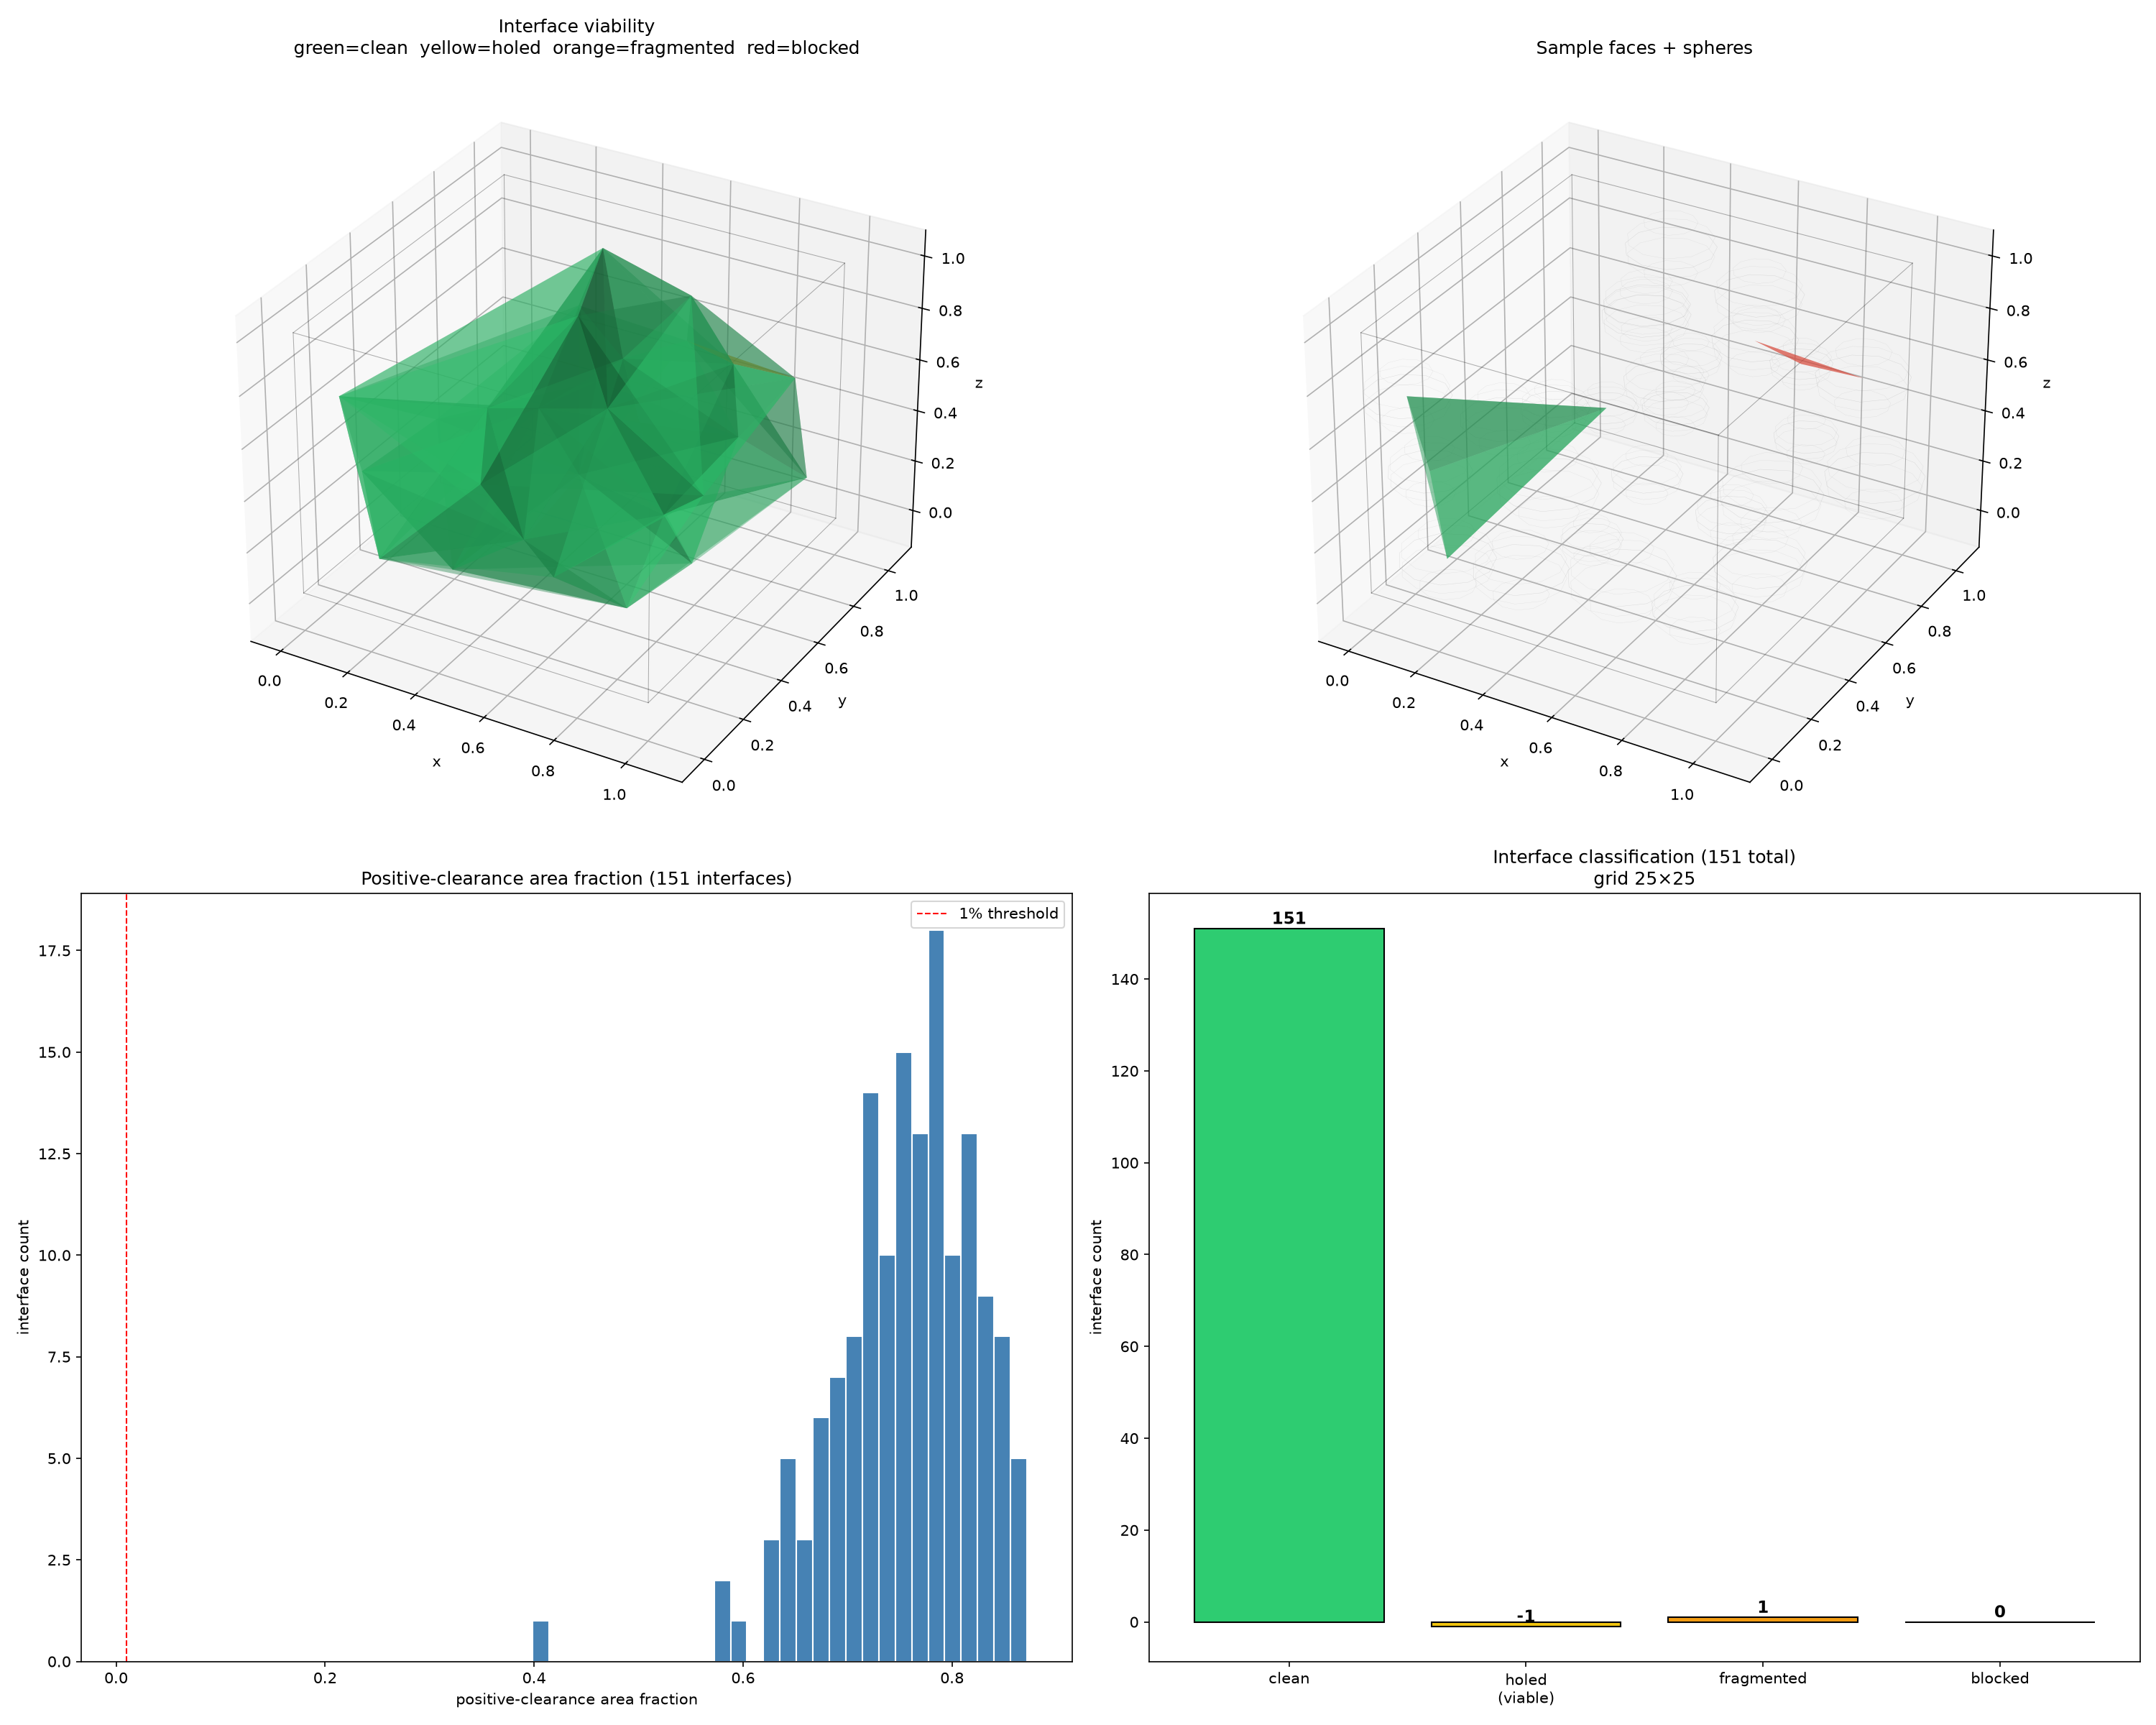
\includegraphics[width=\textwidth]{delaunay_refined_v2.png}
\caption{细化几何正确性筛选结果。\textbf{左上}：界面分类 3D 视图
（绿=clean、黄=holed、橙=fragmented、红=blocked）；\textbf{右上}：代表性面 +
球线框；\textbf{左下}：正 clearance 面积比直方图（红线=1\% 阈值）；
\textbf{右下}：分类柱状图。150/151 面 clean，1 面 fragmented，0 面 blocked，
0 面有 4th 球侵入。}
\label{fig:refined}
\end{figure}

\begin{figure}[htbp]
\centering
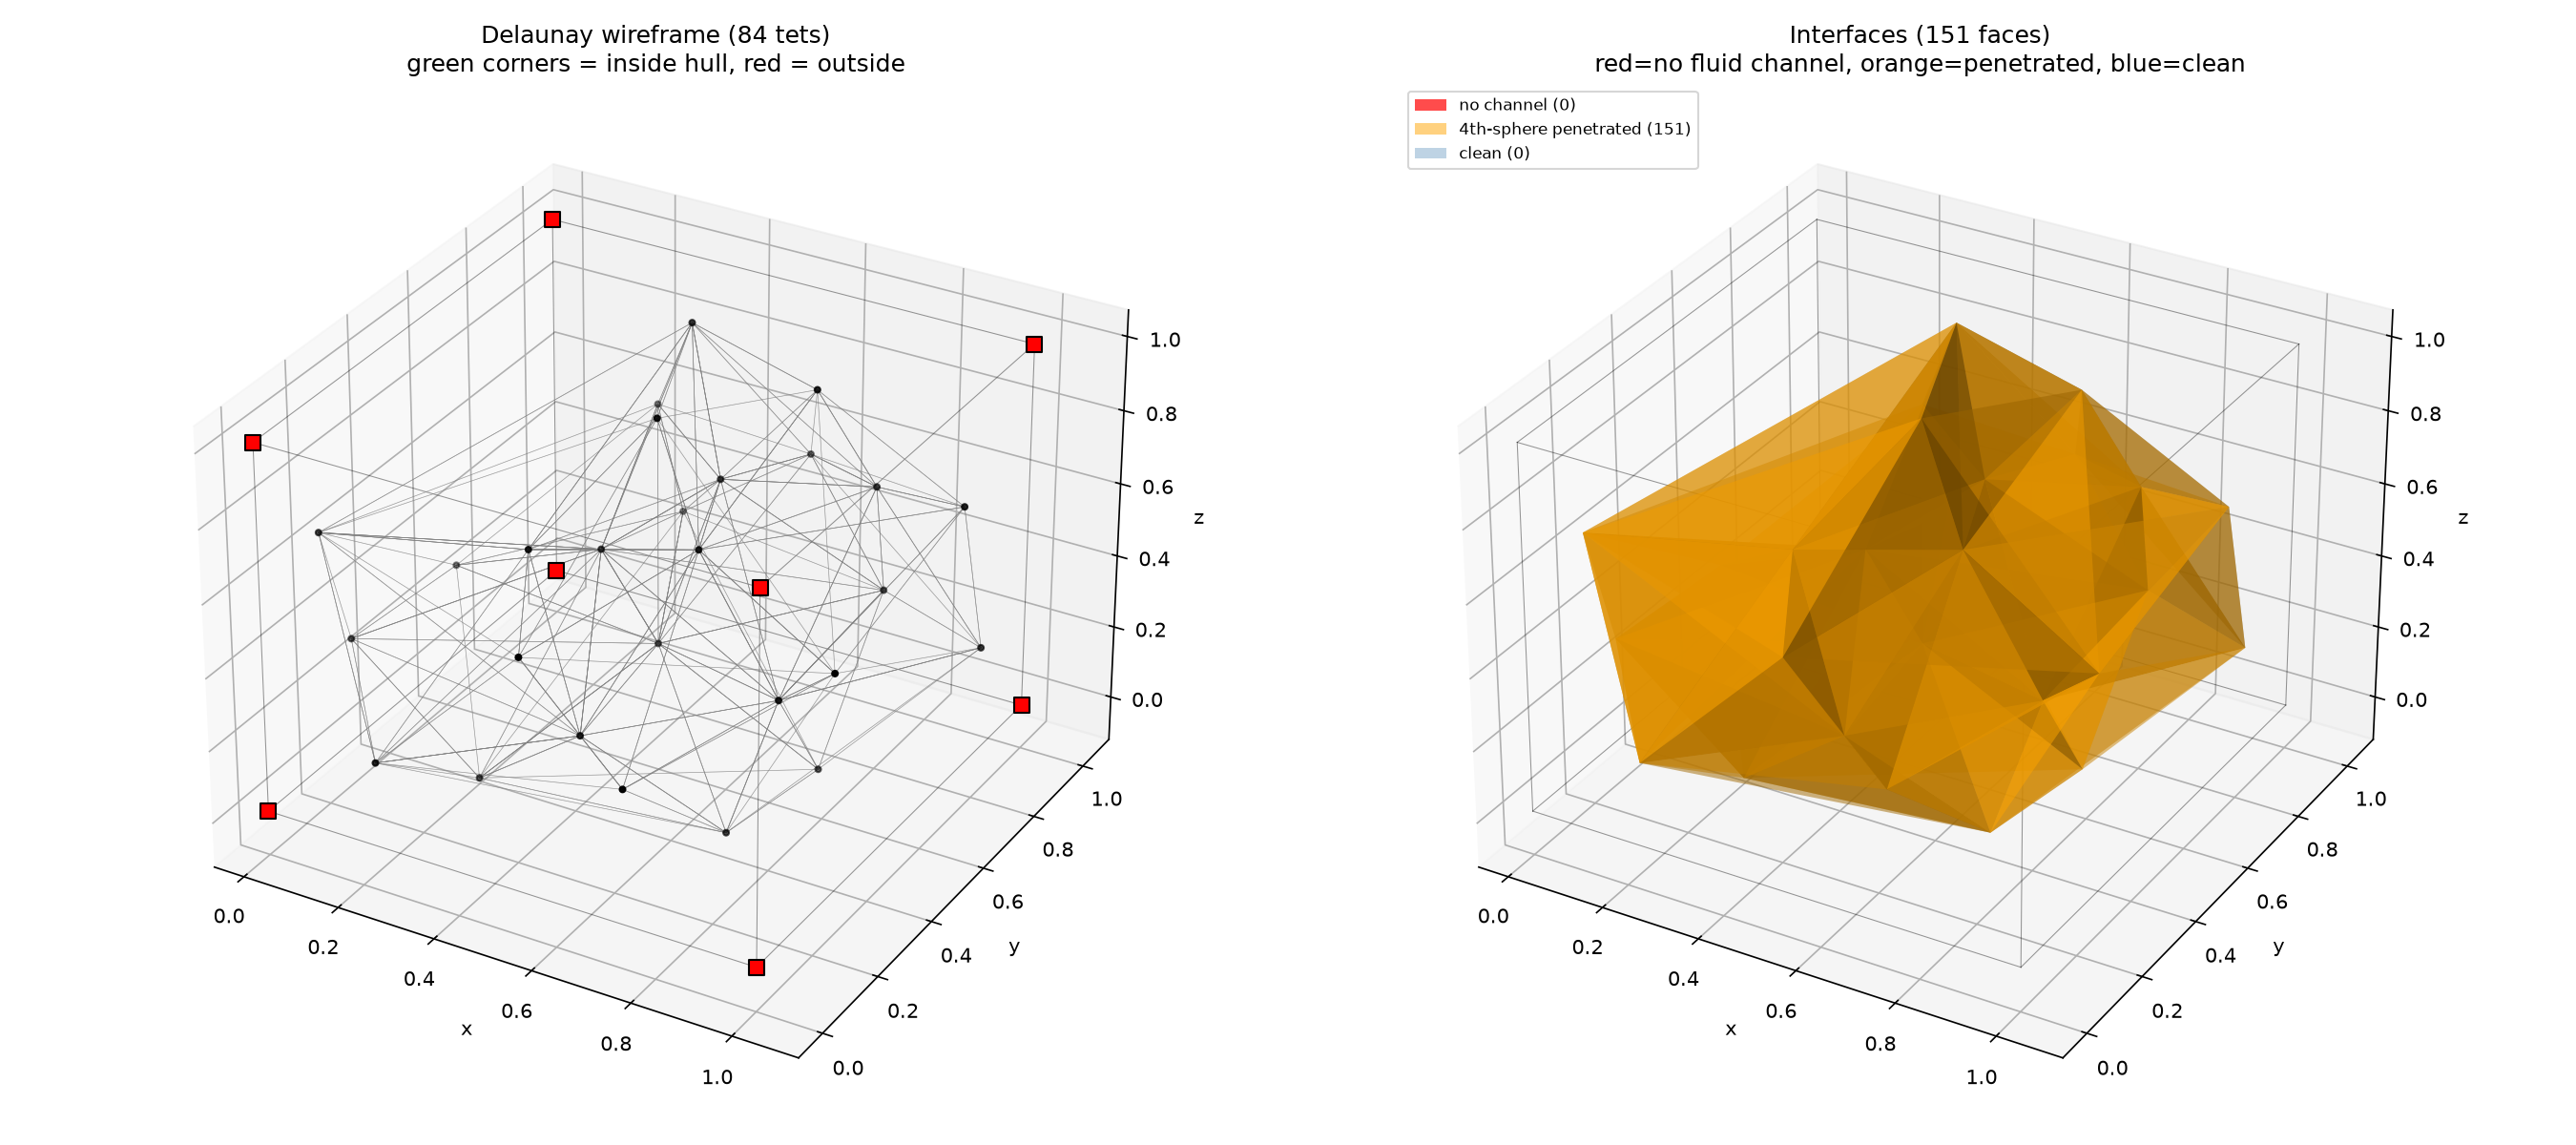
\includegraphics[width=0.75\textwidth]{delaunay_partition.png}
\caption{v1 基础视图。\textbf{左}：Delaunay 骨架（灰线）+ 球心（黑点）+
立方体角（绿=凸包内，红=凸包外）。注意 8 角全红——凸包完全不覆盖立方体。
\textbf{右}：界面三角形着色（蓝=clean、橙=v1 粗口径穿面、红=无通道）。}
\label{fig:partition}
\end{figure}

\begin{figure}[htbp]
\centering
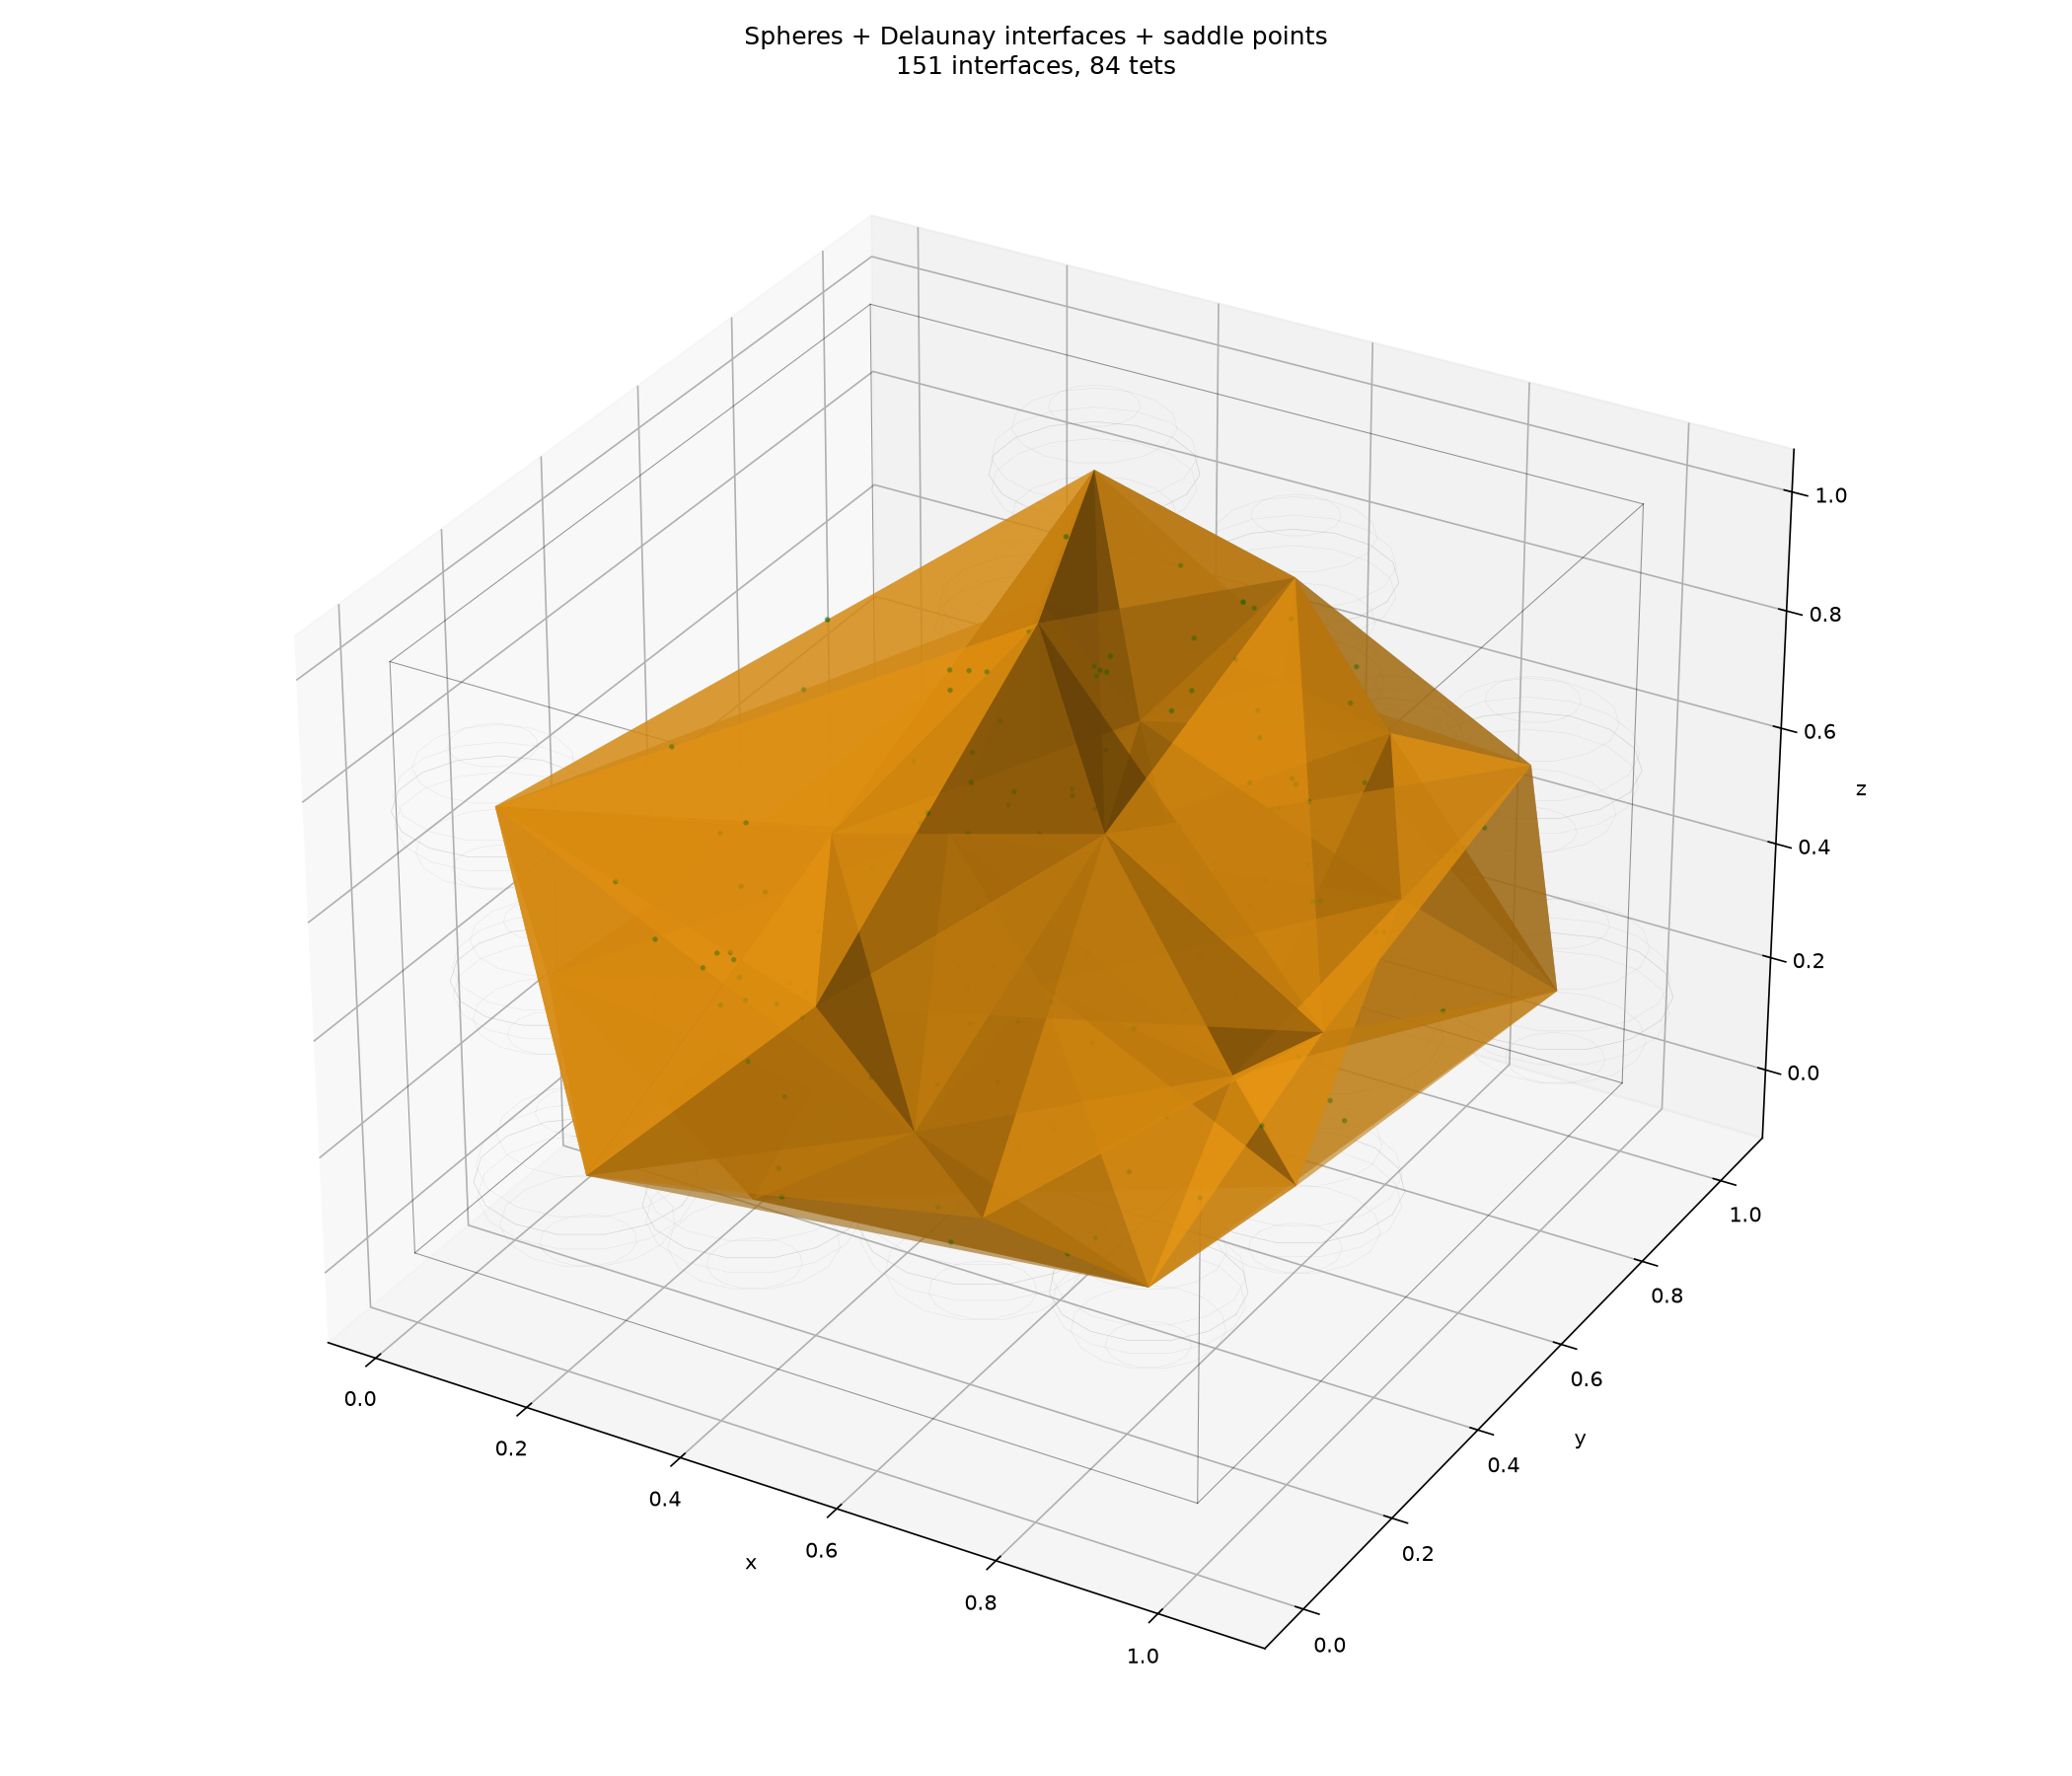
\includegraphics[width=0.9\textwidth]{delaunay_spheres_interfaces.png}
\caption{球线框 + Delaunay 界面 + 鞍点。蓝三角=clean 面，橙=penetrated 面，
红=blocked 面，深绿点=每面鞍点（最大 clearance 位置）。鞍点在球间隙的宽敞
处（$\sim$0.16），不在喉道（$\sim$0.007）。}
\label{fig:spheres}
\end{figure}

\section{两个声称的缺陷及其可修复性}

\subsection{缺陷 A："constriction 极薄，网格化不可行" $\longrightarrow$ 伪缺陷}

初检发现正 clearance 区域的 constriction（最小正 clearance）中位仅 $4.8\times
10^{-4}$，引出了"需要局部 $h<0.0005$ 网格"的担忧。\textbf{这是 metric artifact}：

\begin{itemize}
  \item 正 clearance 区域的边界精确落在 3 个顶点球的圆盘边缘，那里 $d(P)\equiv0$；
  \item constriction 测量的只是"离边界最近的采样点"的 clearance——采样越密越
  接近 0，不是通道真的窄；
  \item 实际通道面积充足（中位 76.4\%）。
\end{itemize}

\textbf{绕过}：用 mesh labeling（如 watershed 的胞标记方式）而非嵌面（OCC
fragment），界面落在网格 facet 上，constriction 被网格尺度吞掉，不做额外细化。
代价是接口变阶梯状（和 watershed 同病）。

\textbf{判定}：\textbf{可绕过。不是本质缺陷。}

\subsection{缺陷 B："界面偏离真喉道 21$\times$" $\longrightarrow$ 不可修复的本质缺陷}

Delaunay 面必须穿过 3 个球心（这是 Delaunay 剖分的几何定义）。球心在固体内部，
而物理喉道在球与球之间的间隙里。规则情形靠立方晶格对称性巧合地让鞍点落在坐标
平面上——随机几何没有对称性。

\textbf{为何不能靠删面（胞合并）修复}：删面改变的是拓扑（哪些胞并成一个），不改
变剩余界面的几何位置。合并后剩余的 Delaunay 面仍然穿过球心，仍然在孔体内部而
非喉道。设法把界面从球心平面"移到"喉道位置等价于放弃 Delaunay 面的定义——即
放弃"平凡方法"本身。

\textbf{判定}：\textbf{不可修复。这是方法的定义性缺陷。}

\begin{verdictbox}
\textbf{最终判定}：Delaunay 四面体剖分在随机几何上\textbf{几何自洽但不可用于
DDPNM}。子区域可以画出来（150/151 面有连通流体通道、0 个 4th 球侵入），但
界面系统性地位于孔体内部而非喉道最窄处——这是 Delaunay 剖分钉子球心晶格上
的必然代价，不可用拓扑微调修复。
\end{verdictbox}

\section{与其他方法的定位}

\begin{table}[htbp]
\centering
\caption{四种分区方法的比较}
\label{tab:comparison}
\small
\begin{tabularx}{\textwidth}{lccccX}
\toprule
方法 & 界面位置 & 接口光滑度 & 预期精度 & 可行性\\
\midrule
Voronoi（嵌面） & 喉道（0.007）& 平面 & 6.5\%（Affine）& 可行\\
Watershed（labeling）& 鞍面 & 阶梯 & 11.3\%（Affine）& 可行\\
Delaunay（嵌面）& \textbf{孔体（0.157）} & 平面 & --- & 不可网格化\\
Delaunay（labeling）& \textbf{孔体（0.157）} & 阶梯 & $>11.3\%$（推测）& 精度无优势\\
\bottomrule
\end{tabularx}
\end{table}

Delaunay 在任何一个维度上都不优于现有方法——界面位置错误或接口质量差，二者必居
其一。

\section{论文使用建议}

这是一个\textbf{有价值的负结果}，可直接进入论文第 2 章"升维的几何断裂"。
建议措辞：

\bigskip

\begin{keybox}{论文素材：第 2 章"机械搬用二维逻辑"段落}
在随机几何中，过球心平面族的最小闭胞是球心点集的 Delaunay 四面体剖分（84 胞、
151 界面）。几何正确性检查（$25\times25$ 采样/面）表明所有界面都有连通的流体
通道（正 clearance 面积比中位 76.4\%），且无任何 4th 球侵入（v1 粗口径"151/151
穿面"经几何交集细化后归零）。然而，界面穿过球心，鞍点净距中位 0.157，是 Voronoi
垂直平分面（0.0073）的 21.5 倍——界面系统性地位于孔体内部而非喉道最窄处。规则
情形的晶格对称性（鞍点恰好落在坐标平面上）在随机几何中完全失效，且此缺陷无法
通过胞合并等拓扑微调修复——它是 Delaunay 剖分的几何定义决定的。因此，三维随机
几何的子区域构造不能机械搬运二维/规则情形的"过球心平面"逻辑，必须重新发明
（第 3--4 节的 Voronoi 与 watershed 方法）。
\end{keybox}

\textbf{定位}：作为叙事中"平凡推广失败 $\to$ 被迫发明新方法"的动机锚点。与
§2.1 的例 2（两不等半径球、Voronoi 偏离 $|r_i-r_j|/2$）和例 4（规则阵列 64 vs
27）形成互补——例 2 说明 Voronoi 的偏离是 $O(|r_i-r_j|)$ 量级，本文说明 Delaunay
的偏离是 $O(1)$ 量级（完全错误的位置）。

\section{源码与数据}

\begin{itemize}
  \item \textbf{分析脚本}：
  \texttt{affine\_ddpnm\_3d\_random\_porous/delaunay\_feasibility.py}（v1 粗口径）、
  \texttt{delaunay\_feasibility\_v2.py}（v2 细化几何交集筛选）；
  \item \textbf{JSON 数据}：
  \texttt{outputs/delaunay\_feasibility/delaunay\_report\_v2.json}（每面详细指标）；
  \item \textbf{全部图片}：
  \texttt{outputs/delaunay\_feasibility/} 目录下
  \texttt{delaunay\_refined\_v2.png}、
  \texttt{delaunay\_partition.png}、
  \texttt{delaunay\_spheres\_interfaces.png}、
  \texttt{delaunay\_dummies\_and\_saddles.png}；
  \item \textbf{本文档 \TeX{} 源码}：
  \texttt{deepseekoutput/delaunay\_feasibility\_verdict.tex}。
\end{itemize}

\end{document}
